
%(BEGIN_QUESTION)
% Copyright 2006, Tony R. Kuphaldt, released under the Creative Commons Attribution License (v 1.0)
% This means you may do almost anything with this work of mine, so long as you give me proper credit

A very interesting form of liquid level switch exploits an optical principle known as {\it Snell's Law}, which relates the angle of a light beam as it passes from one transparent medium to another to the velocities of light in both media:

$$\includegraphics[width=15.5cm]{i00305x01.eps}$$

$${{\sin \theta_1} \over v_1} = {{\sin \theta_2} \over v_2}$$

In this example, which material has the faster velocity of light?  How can you tell?

\vskip 10pt

Something interesting happens when we increase the angle of $\theta_1$.  At some point, $\theta_2$ increases to equal 90$^{o}$, at which point the light never leaves the first medium, but experiences {\it total internal reflection}:

$$\includegraphics[width=15.5cm]{i00305x03.eps}$$

Use algebra and trigonometry to solve for the minimum angle $\theta_1$ at which total internal reflection occurs, in terms of $v_1$ and $v_2$.

\vskip 10pt

\filbreak

We exploit this principle in a refractive-type level switch by aiming a light beam at the inside surface of a quartz prism at such an angle that the light will internally reflect when the prism is surrounded by air, but refract (and escape) when the prism is surrounded by water.  This works because the velocities of light in air and water are not equal:

$$\includegraphics[width=15.5cm]{i00305x02.eps}$$

Identify what else is needed in this optical system to make a complete, working switch, and identify process fluids that would work well with this form of switch.

\vskip 20pt \vbox{\hrule \hbox{\strut \vrule{} {\bf Suggestions for Socratic discussion} \vrule} \hrule}

\begin{itemize}
\item{} Examining the various illustrations shown, identify which of the materials at the interface possesses the greatest {\it dielectric permittivity}.
\end{itemize}

\underbar{file i00305}
%(END_QUESTION)





%(BEGIN_ANSWER)

%(END_ANSWER)





%(BEGIN_NOTES)

The relative velocities of light shown in the example may be determined by analyzing the relative sine values.  Since $\theta_2$ is clearly greater than $\theta_1$, and both angles less than 90$^{o}$, $\sin \theta_2$ must likewise be greater than $\sin \theta_1$.  If this is true, and both fractions are equal to each other, $v_2$ must be greater than $v_1$:

$$v_1 < v_2$$

\vskip 10pt

The minimum angle for total internal reflection may be found by determining the necessary angle $\theta_1$ to make $\theta_2$ equal to 90$^{o}$:

$${{\sin \theta_1} \over v_1} = {{\sin \theta_2} \over v_2}$$

$${{\sin \theta_1} \over v_1} = {{\sin 90^o} \over v_2}$$

$${{\sin \theta_1} \over v_1} = {1 \over v_2}$$

$$\sin \theta_1 = {v_1 \over v_2}$$

$$\theta_1 = \sin^{-1} \left( {v_1 \over v_2} \right)$$

\vskip 10pt

A {\it light detector} is needed to complete the optical switch.

\vskip 20pt

% No blank lines allowed between lines of an \halign structure!
% I use comments (%) instead, so that TeX doesn't choke.

$$\vbox{\offinterlineskip
\halign{\strut
\vrule \quad\hfil # \ \hfil & 
\vrule \quad\hfil # \ \hfil \vrule \cr
\noalign{\hrule}
%
% First row
{\bf Substance} & $n_D$ at 20 $^{o}$C \cr
%
\noalign{\hrule}
%
% Another row
Carbon bisulfide & 1.62546 \cr
%
\noalign{\hrule}
%
% Another row
Ethanol (Ethyl alcohol) & 1.36048 \cr
%
\noalign{\hrule}
%
% Another row
Methyl ethyl ketone & 1.3788 \cr
%
\noalign{\hrule}
%
% Another row
Methyl vinyl sulfone & 1.4636 \cr
%
\noalign{\hrule}
%
% Another row
Pentane & 1.3575 \cr
%
\noalign{\hrule}
%
% Another row
Toluene (Methyl benzene) & 1.4961 \cr
%
\noalign{\hrule}
%
% Another row
Water & 1.33299 \cr
%
\noalign{\hrule}
} % End of \halign 
}$$ % End of \vbox


The process liquid must have a velocity of light less than that of the gas or vapor above the process level in order to halt total internal reflection when liquid contacts the prism.  If the liquid's optical velocity is too high, total internal reflection will continue even with that liquid touching the prism.  Also, the liquid must be transparent and not ``foul'' the surface of the prism.

\vskip 10pt

An {\it index of refraction} is a ratio of the speed of light through vacuum compared to the speed of light through a particular substance.  The greater the index of refraction, the slower the speed of light through that substance:

$$n = {c \over v}$$

\noindent
Where,

$n$ = Index of refraction

$c$ = Speed of light in a vacuum ($\approx$ 3 $\times$ 10$^{8}$ m/s)

$v$ = Speed of light through the particular substance

\vskip 20pt

Indices of refraction taken from the {\it CRC Handbook of Chemistry and Physics}, 64$^{th}$ edition.







\vfil \eject

\noindent
{\bf Summary Quiz:}

A beam of light will refract (bend) when it passes at an angle through materials having different:

\begin{itemize}
\item{} Colors or transparencies
\vskip 5pt 
\item{} Mass densities
\vskip 5pt 
\item{} Temperatures
\vskip 5pt 
\item{} Velocities of light
\vskip 5pt 
\item{} Electrical resistance
\vskip 5pt 
\item{} Magnetic permeabilities
\end{itemize}

%INDEX% Switch, level: optical refraction
%INDEX% Physics, optics: refraction and Snell's Law

%(END_NOTES)


